\documentclass{article}
% \usepackage[utf8]{inputenc}

% Language and font encodings
\usepackage[brazil]{babel}
\usepackage[T1]{fontenc}
\usepackage{ae}

% Sets page size and margins
\usepackage[a4paper,top=3cm,bottom=2cm,left=1cm,right=1cm,marginparwidth=1.75cm]{geometry}

% Useful packages
\usepackage{amsmath,amsthm,amssymb,amsfonts}
\usepackage{graphicx}
\usepackage[colorlinks=true, allcolors=blue]{hyperref}
\usepackage{algorithm}
\usepackage[noend]{algpseudocode}

\usepackage{float}

% Useful commands
% % Math
\newcommand{\R}{\mathbb{R}}
\newcommand{\N}{\mathbb{N}}
\newcommand{\Z}{\mathbb{Z}}
\newcommand{\C}{\mathbb{C}}
\newcommand{\fourier}{\mathfrak{F}}
\DeclareMathOperator{\PS}{PS}
\newcommand{\st}{\ \text{tal que}\ }
\newcommand{\tq}{\ \text{tal que}\ }
\DeclareMathOperator{\SSE}{SSE}
\newcommand{\Loss}{\mathcal{L}}
\newcommand{\e}{\mathbf{e}}
% % Differentials
\newcommand{\diff}[1]{\frac{\mathrm{d}}{\mathrm{d}#1}}
\newcommand{\pdiff}[1]{\frac{\partial}{\partial #1}}
% % Text
\newcommand{\ie}{i.e.\ }
\newcommand{\eg}{e.g.\ }
% % Misc
\newcommand{\note}[1]{{\color{red}{\bf Note:} #1}}
\newcommand{\todo}[1]{{\color{blue}{\bf TO DO:} #1}}

\title{Relatório -- Trabalho Final \\
       \large Estrutura de Dados e Algoritmos -- 2021 -- Prof. Jorge Poco}
\author{Daniel Csillag \\ Rafael Portacio \\ Wellington José}

\begin{document}
\maketitle

\section{Introdução}
Aqui gostaríamos de criar um Waze da cidade do Rio de Janeiro usando algoritmos diferentes de busca para encontrar o menor caminho entre dois pontos dados. 

\section{Coleta e armazenamento dos dados}

Assim como foi especificado na proposta do projeto, extraímos os dados usando a biblioteca OSMnx. Com eles criamos um arquivo \textsc{.json} com as informações dos nós (id, latitude e longitude) e das arestas (nó de saída, nó de chegada, comprimento e tempo estimado de chegada [ETA]). Fazemos uma leitura desse \textsc{.json} em código \textsc{c++} criar o objeto grafo, que contém objetos arestas e nós. Organizamos os nós num \textsc{hash map}. Para as arestas, fizemos uma lista de adjacências (adjacency list) já que temos um grafo bem esparso (pois os graus dos nós são pequenos em relação à quantidade de nós total). Dessa forma, teríamos que uma matriz de adjacências seria desnecessariamente grande pois teria dimensões extremamente altas e a grande maioria dos elementos dela seriam iguais a zero.

\section{Backend}

Aqui usamos os algoritmos Dijsktra, A* com heurística euclidiana e A* com heurística manhattan. Usando uma \textsc{min heap} que implementamos para gerenciar os custos dos caminhos. \\

A principal diferença do dijkstra para o A* é a adição da heurística que está implementada como uma função que é passada como argumento para o algoritmo e cuja a utilidade é dar prioridade para os nós que se aproximam do destino final, chegando assim no destino final com menos passos.

\section{Frontend}

\begin{figure}[H]
    \centering
    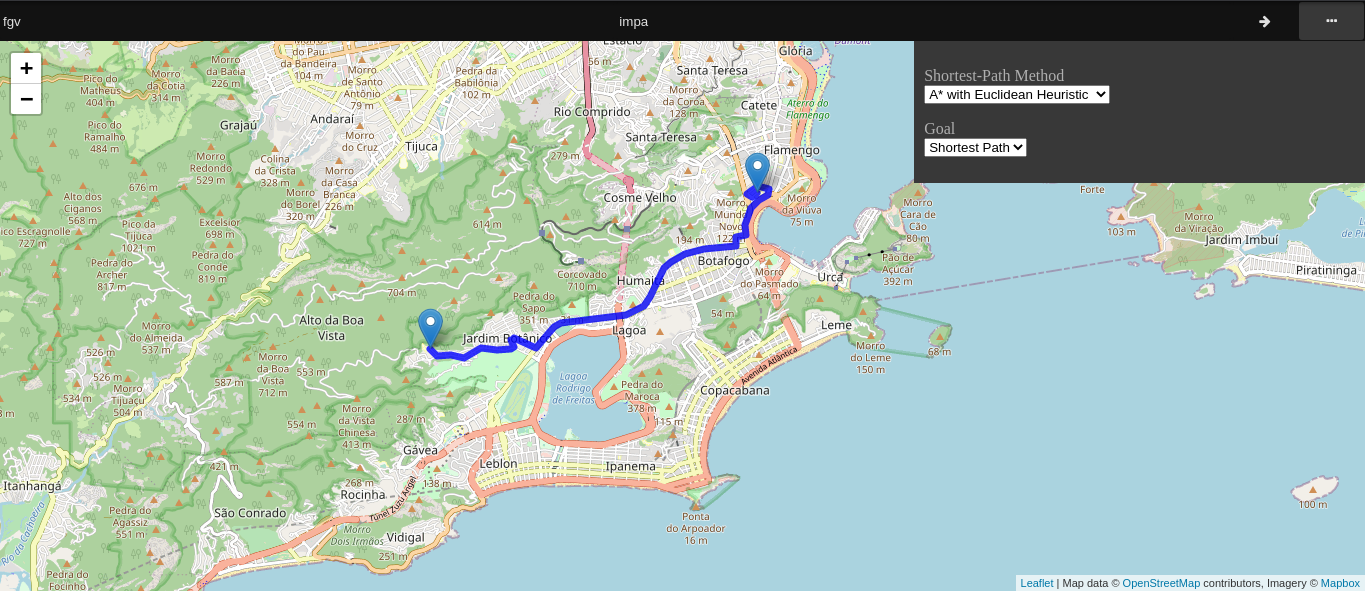
\includegraphics[scale=0.53]{EDA_full_inteface_web.png}
    \caption{Caption}
    \label{fig:my_label}
\end{figure}

No Frontend, colocamos algumas features, tais como:
\begin{itemize}
    \item permitir a escolha do algoritmo a ser utilizado a partir de uma dropdown.
    
    \item poder selecionar os pontos de início e fim a partir da função de geocoding do nominatim, assim permitindo escrever endereços para obter os pontos.
    
    \item poder mudar os pontos de início e fim ao arrastar seus respectivos markers pelo mapa.
    
    \item armazenar na url as coordenadas de início e fim, assim como o algoritmo utilizado, para assim poder obter o mesmo trajeto ao copiar a url para outra aba.
    
    \item exibir o comprimento, o tempo estimado de chegada e o tempo de execução do algoritmo utilizado ao posicionar o mouse sobre um dado caminho.
    
    \item podemos calcular não só o menor caminho como também o mais rápido a partir de uma dropdown. Logo abaixo temos os 2 casos:
    
\begin{figure}[H]
    \centering
    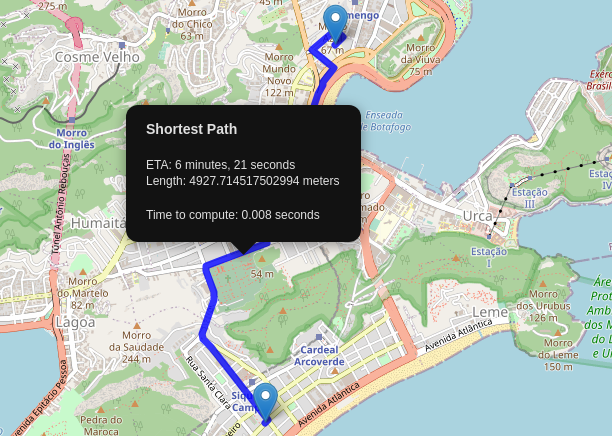
\includegraphics[scale=0.74]{EDA_path_with_shortest_path.png}
    \caption{Caminho com distancia}
    \label{fig:my_label}
\end{figure}

\begin{figure}[H]
    \centering
    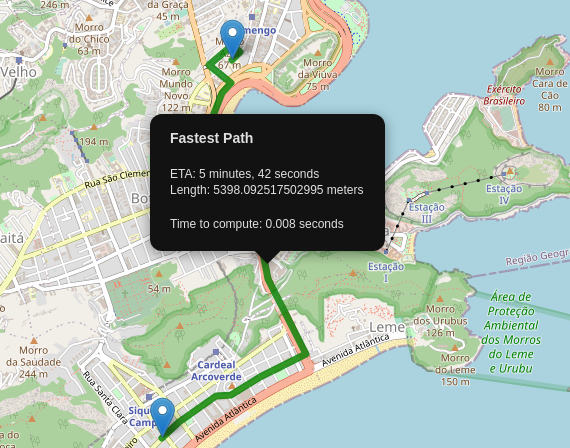
\includegraphics[scale=0.8]{EDA_path_with_fastest_path.png}
    \caption{Caminho com menor tempo}
    \label{fig:my_label}
\end{figure}

\end{itemize}

\section{Problemas encontrados}

Conforme testamos, encontramos problemas no Waze que tínhamos:
\subsection{Lookup pelo nó mais próximo}
No início, nossa implementação encontrava o nó mais próximo dos pontos de início e de fim, mas nisso encontramos problemas, pois assim só podíamos traçar caminhos conectando nós e por mais que adicionássemos uma conexão do ponto de início ao primeiro nó e do ponto de final ao segundo nó, essa conexão poderia ser estranha ou até mesmo um trajeto contramão.

Visando resolver isso, nós implementamos uma busca pela aresta mais próxima e projetamos o ponto nela, e com essa aresta podemos fazer a conexão do ponto de início a um nó que é adequado para ele se conectar.

\subsubsection{Tomando frações de arestas}
No caso, para conectar o ponto de início a um nó, pode ser que precisemos fazer um trajeto equivalente a uma fração de uma aresta, e dessa forma adicionamos isso no trajeto, usando para isso um peso(weight) igual à porcentagem de fração tomada vezes o peso total da aresta, sendo assim o peso proporcional à fração. Permitindo assim posicionar pontos no meio das ruas e não somente nos nós. (Conforme imagem abaixo)

\begin{figure}[H]
    \centering
    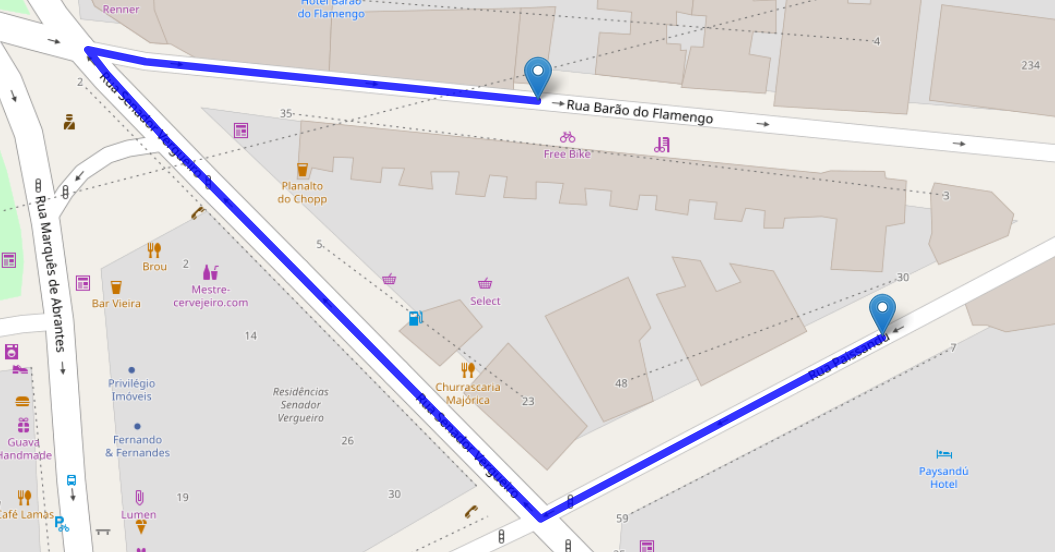
\includegraphics[scale=0.6]{EDAreport-fraction-edge.png}
    \caption{Como podemos ver aqui temos pontos que não são vértices}
    \label{fig:my_label}
\end{figure}

\subsection{Ruas com mão dupla}
Quando por exemplo o início está no meio de uma rua de mão dupla, existem duas opções para o nó de início do trajeto e por isso faz-se necessário chamar o algoritmo mais de uma vez caso deseje-se usar o grafo original. Sendo em alguns casos, necessário chamar o algoritmo 4 vezes, caso ambos o início e fim estejam no meio de ruas de mão.\\
\textbf{OBS:} Uma possibilidade para evitar que o algoritmo seja chamado mais de uma vez, seria usar um grafo alterado G' em que temos os nós do pontos de início e fim adicionados no grafo e fazemos as mudanças necessárias.\\

Na nossa implementação atual, temos um bug para ruas de mão dupla, por ele acabar percorrendo até o ponto final depois de passar pela mesma rua onde ele está. (Conforme imagem abaixo)

\begin{figure}[H]
    \centering
    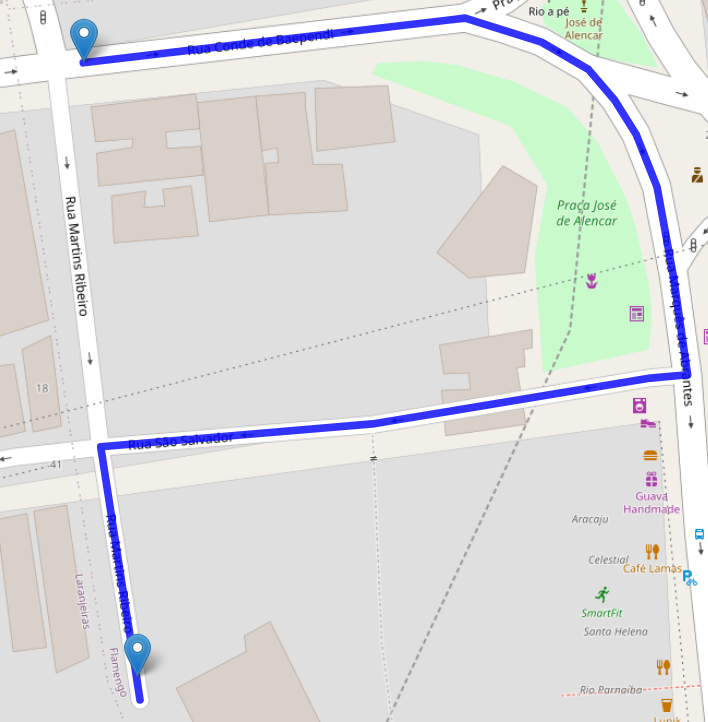
\includegraphics[scale=0.59]{EDAreport-two-way-street-bug.png}
    \caption{Caption}
    \label{fig:my_label}
\end{figure}

\section{Conclusão}
...

\end{document}
